\section{Introduction}
This research introduces a new system that combines clear step-by-step planning, long-term memory, and multiple specialized agents working together. Unlike older models that rely completely on expensive cloud services, this new design focuses on doing as much work as possible locally on the user's machine. By handling most decisions and tasks locally, the system runs more smoothly, uses fewer tokens, and costs much less to operate.

To make this work, the system avoids messy, open-ended conversations. Instead, it uses a strict, organized method to complete tasks. At the heart of this system is a smart filtering process. When a user makes a request, the system first tries to understand and solve it using fast, local AI models. It only sends the request to large, expensive cloud models if the task requires deep thinking or complex problem-solving. This ensures that expensive cloud models are not wasted on simple tasks.

Additionally, the system is designed to learn from experience. By using local databases, it saves a record of how it successfully completed past tasks, such as writing code or navigating websites. This creates a historical memory, allowing the agent to skip the planning phase when it encounters a similar problem again. As a result, the system becomes faster and more affordable over time as its local knowledge grows.

\section{Key Agent Features}
The proposed agent system includes the following main features:\\
\begin{enumerate}
    \item \textbf{Local Memory:} It uses a local database (ChromaDB) to remember important information, so it does not have to waste time searching for the same files over and over again.
    \item \textbf{Fast Machine Learning:} It uses lightweight tools (FLAML) to quickly optimize and tune the system directly on the user's computer without needing heavy resources.
    \item \textbf{Pre-Built Tool Library:} Common tools and computer commands are saved permanently in a local database, so they are always ready to be used instantly.
    \item \textbf{On-the-Fly Tool Creation:} If the system faces a brand new problem, it can ask the AI to write a new tool. This new tool is then saved into the database so it can be reused later.
    \item \textbf{Smart Local Routing:} A local supervisor program carefully checks every task. It decides whether the task can be handled locally or if it needs to be sent to a cloud AI, saving money and time.
    \item \textbf{Step-by-Step Fallback:} If the local supervisor cannot understand a request, it tries a small local AI model first. It only sends the request to a large, expensive cloud AI as an absolute last resort.
    \item \textbf{Structured JSON Plans:} Instead of guessing what to do, the system creates a clear, step-by-step roadmap (saved as a JSON file) before it starts working. This makes the process easy to track and verify.
    \item \textbf{Self-Fixing Plans:} If something goes wrong while following the roadmap, the AI can automatically update and fix the plan to get back on track.
    \item \textbf{Continuous Execution:} Instead of forgetting what it was doing between commands, the system keeps its background processes running. This helps it remember the current state of the computer environment.
    \item \textbf{Browser Recording:} When the agent uses a web browser, it records its actions. If it needs to do the same task again, it simply replays the recording instead of asking the AI to figure it out twice.
    \item \textbf{Smart Error Reading:} When testing code, error logs can be extremely long. The system automatically shortens these logs and only shows the most critical errors to the AI, which saves tokens and prevents confusion.
\end{enumerate}

\begin{figure}[H]
    \centering
    \vspace{-3cm}
    
\includegraphics[width=0.63\textwidth]{images/ecogent_workflow.png}
    \caption{Ecogent Architecture Workflow.}
    \label{fig:ecogent_workflow}
\end{figure}

As illustrated in Figure \ref{fig:ecogent_workflow}, the system follows a clear, multi-step process to handle user requests efficiently and affordably. The workflow begins the moment a user submits a prompt or task. Instead of sending this request directly to an expensive cloud AI, the system first routes the input to the Local NLP Supervisor. This supervisor acts as a fast and intelligent filter. It quickly analyzes the user's intent and searches the local database (ChromaDB) to see if the system already has the right tools or a past solution for this exact problem.\\

If the task is simple or has been solved before, the supervisor matches it with the correct local tool. The system then executes the task entirely on the user's local machine. This means the task is completed instantly and at absolutely zero cost, because no cloud APIs were used.\\

However, if the request is slightly more complicated and the supervisor cannot find a direct match, the system moves to the second step: the local Tiny LLM. This is a very small, lightweight AI model (for example, a 135-million parameter model) that runs directly on the local computer. It tries to understand the request and generate a solution without needing an internet connection. Because it is small, it runs very quickly and still costs nothing in terms of cloud API fees.\\

Finally, if the user's request is highly complex and both local layers fail to solve it, the system reaches the third step: cloud escalation. Rather than defaulting to the most expensive model every time, future implementations of Ecogent will use a dynamic difficulty score to route the task to either a low-cost, mid-cost, or high-cost Cloud LLM. For instance, a moderately difficult task might be sent to a cheaper cloud model, while only the most extremely difficult tasks are sent to massive models like GPT-4 or Claude. By using this step-by-step filtering process, the system guarantees that expensive cloud models are only used when absolutely necessary. This smart routing drastically cuts down on operational costs while still providing top-tier AI performance for difficult problems.\\

\begin{figure}[H]
\centering
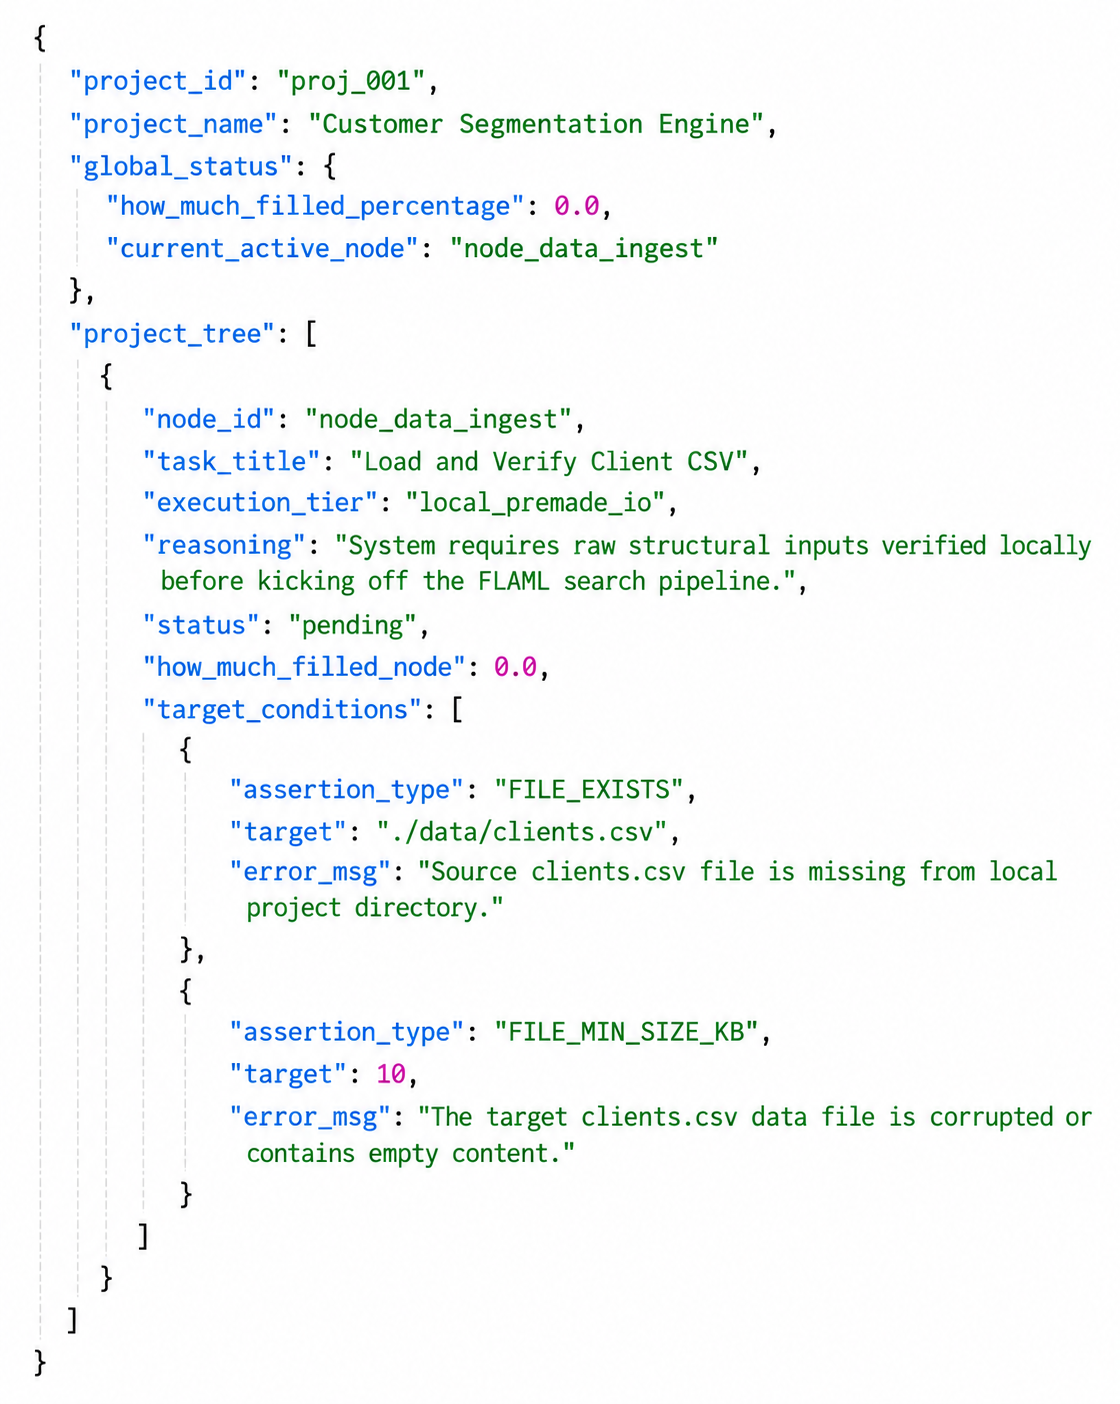
\includegraphics[width=1\textwidth]{images/ecogent_project_json.png}
\caption{Example Project Planning JSON.}
\label{fig:project_json}
\end{figure}

Furthermore, as seen in Figure \ref{fig:project_json}, once a complex workflow is planned, the system breaks it down into a highly structured JSON tree rather than maintaining an unstructured conversation history. This declarative plan dictates the exact sequence of sub-tasks and verification conditions required for execution.



\begin{algorithm}[H]
\caption{JSON Project Tree Execution and Verification}
\begin{algorithmic}[1]
    \State \textbf{Output:} Updated Execution State \& Evaluated Nodes
    
    \State $Tree \gets P.\text{project\_tree}$
    \State $GlobalStatus \gets P.\text{global\_status}$
    
    \For{\textbf{each} $node \in Tree$}
        \If{$node.\text{status} == \text{"pending"}$}
            \State $GlobalStatus.\text{current\_active\_node} \gets node.\text{node\_id}$
            \State \text{Execute task via } $node.\text{execution\_tier}$
            \State $VerificationPassed \gets \text{True}$
            
            \Statex \qquad \textbf{\% Evaluate Target Conditions}
            \For{\textbf{each} $cond \in node.\text{target\_conditions}$}
                \If{$cond.\text{assertion\_type} == \text{"FILE\_EXISTS"}$}
                    \State $Valid \gets \text{CheckExists}(cond.\text{target})$
                \ElsIf{$cond.\text{assertion\_type} == \text{"FILE\_MIN\_SIZE\_KB"}$}
                    \State $Valid \gets \text{CheckMinSize}(cond.\text{target})$
                \ElsIf{$cond.\text{assertion\_type} == \text{"CSV\_COLUMN\_EXISTS"}$}
                    \State $Valid \gets \text{CheckColumn}(cond.\text{target.file}, cond.\text{target.col})$
                \EndIf
                
                \If{\textbf{not} $Valid$}
                    \State \textbf{Raise Exception:} $cond.\text{error\_msg}$
                    \State $VerificationPassed \gets \text{False}$
                    \State \textbf{Break}
                \EndIf
            \EndFor
            
            \Statex \qquad \textbf{\% Update Node Status}
            \If{$VerificationPassed$}
                \State $node.\text{status} \gets \text{"completed"}$
                \State $node.\text{how\_much\_filled\_node} \gets 1.0$
            \EndIf
        \EndIf
    \EndFor
    
    \State $GlobalStatus.\text{how\_much\_filled\_percentage} \gets \text{CalculateTotal}(Tree)$
\end{algorithmic}
\end{algorithm}



\subsection{Comparison Between Ecogent and Cloud-Native Agent}
To show the benefits of this new system, this section compares the local-first Ecogent model with traditional cloud-based agents (like Claude Code or Antigravity). The table below highlights the main differences in how they operate, including their core designs and how they handle tasks.\\

\begin{table}[H]
\centering
\resizebox{\textwidth}{!}{%
\begin{tabular}{|p{0.25\linewidth}|p{0.35\linewidth}|p{0.35\linewidth}|}
\hline
\textbf{Dimension} & \textbf{Proposed Local-First (Ecogent)} & \textbf{Cloud-Native (e.g., Claude Code, Antigravity)} \\ \hline
\textbf{System Design} & Uses Local Processing: Tries to solve problems locally first; uses the cloud only when absolutely necessary. & Relies on the Cloud: Sends almost all thinking and planning directly to expensive cloud models. \\ \hline
\textbf{Finding Files} & Smart File Memory: Instantly finds files using a local database (ChromaDB), preventing the AI from getting lost or guessing wrong paths. & Constant Searching: Has to search through folders repeatedly using slow commands, which wastes time and tokens. \\ \hline
\textbf{Web Browsing} & Record and Replay: Records step-by-step browser actions and replays them for free on similar tasks. & Reads from Scratch: Forces the AI to read and understand the entire web page again every single time. \\ \hline
\textbf{System Commands} & Continuous Memory: Keeps background terminal windows open so it remembers its location and what it was doing. & Forgetful Execution: Runs commands that close immediately, causing the AI to easily lose its place. \\ \hline
\textbf{Testing Code} & Smart Error Shortening: Runs tests in the background and only shows the most important errors to save tokens. & Dumping Full Errors: Copies massive error logs directly into the AI, which heavily increases costs. \\ \hline
\textbf{Filtering Tasks} & Step-by-Step Triage: Uses a fast local filter, then a small local AI, and only calls the cloud as a last resort. & Direct to Cloud: Sends the user's raw message straight to a massive, expensive cloud model every time. \\ \hline
\textbf{Creating New Tools} & Save for Later: Automatically writes missing tools and saves them into the local database for future use. & Temporary Code: Writes temporary code snippets inside the chat window that are forgotten later. \\ \hline
\textbf{Planning Tasks} & Clear JSON Roadmaps: Creates a strict, step-by-step JSON plan for how to finish the task. & Endless Looping: Uses a conversational loop that constantly checks live output, which can easily get stuck. \\ \hline
\textbf{Tuning Performance} & Local Optimization: Uses lightweight tools (FLAML) to improve performance directly on the user's hardware. & Cloud Reliance: Depends entirely on expensive commercial cloud services to handle optimization. \\ \hline
\textbf{Data Privacy} & Kept Safe Locally: All code, data, and system information stay safely on the user's computer. & Constantly Uploading: Streams the user's private code and data to external cloud servers. \\ \hline
\end{tabular}%
}
\caption{Comparison of Ecogent vs Cloud-Native Architectures}
\label{tab:architecture_comparison}
\end{table}



\subsection{Dual-Database Memory System (ChromaDB + NoSQL)}
Instead of saving long, full chat conversations (which wastes API tokens and drives up cloud costs), the Ecogent system creates short, meaningful "memories" for each task it completes. Think of it like a human taking brief, organized notes instead of recording an entire three-hour meeting word-for-word. When the agent successfully finishes a job, it summarizes the key steps it took and saves them using short, simple tags. 

\textbf{Example Tags:}
\begin{itemize}
    \item \texttt{login\_auth\_fix}
    \item \texttt{checkout\_payment\_error}
    \item \texttt{extract\_invoice\_data}
\end{itemize}

To keep the system lightweight and extremely fast, Ecogent uses a strictly separated, dual-database architecture:
\begin{itemize}
    \item \textbf{Chroma DB (Semantic Search):} A fast, local vector database \cite{chromadb_docs} that acts as the system's index. It stores only tiny semantic keys (embeddings) and minimal metadata. This guarantees zero memory bloat during searches.
    \item \textbf{Local NoSQL JSON Database:} A standard, persistent database that stores the heavy data payloads. It permanently stores the massive JSON workflows, recorded browser patterns, full error logs, and complex file maps.
\end{itemize}

When a user asks the agent to do a new task, the local supervisor first asks Chroma DB, "Have we ever solved a problem like this before?" 

If Chroma DB finds a matching semantic tag, it returns an ID. The system then queries the local NoSQL database to instantly retrieve the full, proven JSON steps from its past experience. It does not need to guess, and it does not need to ask the expensive cloud AI for a new plan. This dual-database "semantic memory" eliminates the need to read through massive conversation histories, saving an enormous amount of time and money while guaranteeing the system gets smarter without bloating the search index.\\

\subsection{Multi-Agent System}
To keep the system organized and prevent confusion, complex tasks are divided among specialized sub-agents:
\begin{itemize}
    \item \textbf{Coding Agent} $\rightarrow$ Uses a smart code map in ChromaDB so it always knows exactly where files are located.
    \item \textbf{Browser Agent} $\rightarrow$ Records web interactions into saved patterns to avoid wasting AI tokens on the same web tasks.
    \item \textbf{Testing Agent} $\rightarrow$ Uses smart testing maps and shortens long error logs to save token costs.
    \item \textbf{OS Agent} $\rightarrow$ Keeps background terminal windows open so it remembers its computer environment between steps.
\end{itemize}

\subsection{Coding Agent Architecture: The Semantic Code Map}
Current coding agents often forget where files are located. They rely on slow, expensive searches that confuse the AI and waste tokens. The Ecogent Coding Agent solves this by saving a smart "Code Map" in ChromaDB. Instead of starting blindly every time, the agent asks the local database to instantly find the exact file path. The system then gives only that specific file to the Cloud AI. This greatly reduces token usage and stops the AI from guessing wrong file paths.\\

To make sure this map stays accurate when files are changed by humans, the system uses a three-step updating process:
\begin{itemize}
    \item \textbf{Active Update:} If the agent changes or renames a file itself, it instantly updates the database for free.
    \item \textbf{Background Update:} A local background process watches for manual user changes and quietly updates the database using a tiny local model.
    \item \textbf{Last-Second Check:} Right before asking the Cloud AI, the system quickly checks if the file still exists. If the file is missing, it quickly rebuilds the map.
\end{itemize}

\subsection{Browser Agent Workflow Pattern System}
The Browser Agent uses a special recording system to avoid using the cloud AI for repetitive web tasks. When asked to do something in the browser, the system first checks ChromaDB to see if it has done a similar task on that specific website before.\\

If a matching record is found, the system simply replays the exact steps without calling the cloud AI, which costs nothing. If one of the steps fails during the replay, the AI steps in only to fix that specific mistake. If the system has never seen the task before, it carefully records its own actions step-by-step. It saves these detailed actions as clear JSON files in the NoSQL database, while saving the search tag in ChromaDB so it can replay them for free in the future.\\

\subsection{OS Agent: Vector-Backed Stateful Execution}
Older AI agents run simple computer commands that close instantly, causing the agent to forget its location and freezing the terminal during long tasks. The Ecogent OS Agent solves this by using continuous, state-aware execution. 
\begin{itemize}
    \item \textbf{System File Map:} Important system files are saved in ChromaDB, which completely eliminates slow file searches.
    \item \textbf{Continuous Terminals:} Commands are sent through background terminal windows that stay open. This allows the agent to remember exactly which folder it is working in.
    \item \textbf{Background Tasks:} Long-running tasks, such as starting a web server, are run in the background. This lets the user keep chatting with the agent while the server runs quietly behind the scenes.
\end{itemize}

\subsection{Testing Agent: Token-Optimized QA Architecture}
Older testing agents usually run tests and send the full, raw output directly to the AI. This can waste a massive amount of tokens if the test produces thousands of lines of errors. The Ecogent Testing Agent prevents this by using a smarter, token-saving design:
\begin{itemize}
    \item \textbf{Smart Testing Maps:} All test commands are saved in ChromaDB, so the agent instantly knows how to test the project without guessing.
    \item \textbf{Smart Error Shortening:} If an error log is too long, the agent automatically cuts out the middle section. It only sends the beginning (the command) and the very end (the exact error message) to the AI.
    \item \textbf{Background Testing:} Tests are run quietly in the background, so the system never freezes while waiting for results.
\end{itemize}

To manage all of these agents, a fast local AI acts as the main supervisor. By checking how difficult a task is before asking the cloud, this supervisor saves time and money. It makes sure that expensive cloud models are only used when deep thinking is truly needed.\\

\subsection{Multi-Tier Routing Algorithm}
The algorithm below shows exactly how the Ecogent supervisor filters tasks. It demonstrates how requests are passed through different layers, starting from free local models and only moving up to expensive cloud models if necessary.\\

\begin{algorithm}[H]
\caption{Multi-Tier Triage and Routing Logic}
\label{algo:multi_tier_routing}
\begin{algorithmic}[1]
    \State \textbf{Input:} User Input $U$
    \State \textbf{Output:} Execution Result
    
    \Statex \textbf{\% Tier 1: Fast NLP + ML-Based Local Supervisor}
    \State $Intent, Confidence \gets \text{NLPSupervisor.Classify}(U)$
    \If{$Confidence \ge \text{THRESHOLD\_HIGH}$}
        \State $Tool \gets \text{VectorDB.RetrieveTool}(Intent)$
        \If{$Tool \neq \text{Null}$}
            \State \Return $\text{ExecuteLocal}(Tool, U)$
        \EndIf
    \EndIf
    
    \Statex \textbf{\% Tier 2: Local Tiny Deep Learning Model Fallback}
    \State $Result \gets \text{TinyLocalModel.Infer}(U)$
    \If{$Result.\text{is\_resolved}$}
        \State \Return $Result.\text{output}$
    \EndIf
    
    \Statex \textbf{\% Tier 3: Cloud LLM via LangGraph (Last Resort)}
    \State $JsonPlan \gets \text{CloudLLM.GeneratePlan}(U)$
    \State $\text{StoreWorkflow}(JsonPlan)$ \Comment{Cache for future reuse}
    \State \Return $\text{ExecutePlan}(JsonPlan)$
\end{algorithmic}
\end{algorithm}

\subsection{Tool System}
The system uses a flexible tool library that is designed to grow and learn over time:
\begin{itemize}
    \item \textbf{Pre-Built Tools:} Common actions are permanently saved in the local database so they can be used instantly without thinking.
    \item \textbf{AI-Generated Tools:} If the agent faces a new problem, it writes a custom tool. Once the tool is tested and proven to work, it is saved for the future.
\end{itemize}
Every tool is saved in Chroma DB with a clear, structured description. This allows the local supervisor to automatically find and use the right tool simply by understanding what the user wants to do.\\

\subsection{Experimental Setup and Evaluation Metrics}
To prove that this local-first system is better than traditional models, several strict experiments will be conducted. These tests are designed to directly answer the main questions of this research.\\

\textbf{Baselines for Comparison:}
Ecogent will be tested against popular cloud-based agents. Specifically, it will be compared to standard versions of AutoGPT and a basic LangChain/LangGraph agent that completely relies on expensive models like Claude or GPT-4.\\

\textbf{Evaluation Benchmarks:}
To make sure the tests are fair, the following standard datasets will be used:\\
\begin{itemize}
    \item \textbf{SWE-bench:} Used to test how well the Coding Agent solves real-world programming problems, comparing its smart map system against older, slower file searching methods.
    \item \textbf{WebArena / BrowserGym:} Used to test the Browser Agent, specifically checking how much money is saved by replaying recorded web actions instead of reading the website from scratch every time.
\end{itemize}

\textbf{Core Evaluation Metrics:}
\begin{itemize}
    \item \textbf{Token Usage:} Counting the exact number of tokens used per task to prove that smart memory and error shortening actually save space.
    \item \textbf{Financial Cost (\$):} Calculating the real money spent on API fees during a task, comparing the new multi-step routing system against a cloud-only approach.
    \item \textbf{Execution Speed:} Measuring exactly how long it takes to finish a task, testing if running processes locally in the background is faster than waiting for the cloud.
\end{itemize}

\subsection{Expected Challenges}
While the local-first approach provides significant benefits, it introduces specific challenges that must be addressed:\\
\begin{itemize}
    \item \textbf{Tool Hallucination:} A primary risk is the Tiny LLM confidently hallucinating an incorrect tool. To mitigate this, the architecture relies heavily on the strict, rule-based NLP Supervisor as the first layer. Furthermore, the Testing Agent runs sandboxed validation checks before any destructive commands are executed.
    \item \textbf{Semantic Overlap in Vector Search:} Because Ecogent efficiently separates the heavy JSON payloads into a NoSQL database and only stores semantic keys in ChromaDB, raw memory bloat is fully prevented. However, as hundreds of workflows are saved, similar tasks might develop overlapping semantic meanings, causing ChromaDB to return the wrong tool ID. To prevent this, strict metadata filtering (e.g., tagging domains like "Browser" vs "OS") is used to isolate searches, and the Tiny LLM acts as a secondary validator before execution.
\end{itemize}
